\section{Tutorial de testing}
\label{sect:testing}

En este apartado se indican los pasos a seguir para poder ejecutar los tests de la aplicación sin complicaciones. Se recomienda hacer
la configuración necesaria en un sistema Unix ya que es donde se ha trabajado la aplicación y, más adelante, se indicará hacer uso de mandatos 
específicos de Unix.

\begin{enumerate}
	\item Lo primero es tener el proyecto actualizado. El repositorio debería ser accesible para cualquier usuario en 
            \href{https://github.com/Javiex7/Outsider}{github.com/Javiex7/Outsider}.
	\item Para la ejecución de los tests en indispensable la instalación tanto de Python \cite{installPython} como de Docker \cite{installDocker}.
	\item Con estos programas instalados en el sistema, es necesario acceder al repositorio para la configuración básica.
	\item Dentro del proyecto, son necesarios la instalación de varios elementos en el dispositivo, específicamente Django y los paquetes
	      pertinentes. Para evitar problemas, se recomienda descargar los elementos listados en el ``requirements.txt'' dentro de la carpeta principal
	      ``OutsiderProject''. Esta instalación se puede realizar fácilmente mediante el mandato: 
	      	                
	      pip install -r requirements.txt
	      	      
	\item A continuación, se requiere ejecutar un contenedor en Docker encargado de gestionar el servidor Redis para
	      que se haga uso en los tests. Mediante el siguiente mandato se puede poner en ejecución el servicio:
	      	      
	      docker run --rm -p 6379:6379 redis:7
	      	      
	\item Antes de poder ejecutar los tests, se debe configurar un variable de entorno para indicar el uso de 
	      este servidor Redis. Para ello habría que acceder a ``OutsiderProject/outsider/settings.py'' y modificar
	      el flag booleano denominado ``TEST'' y asegurarse que su valor sea True (línea 92).
	      	      
	\item Finalmente, el sistema puede ejecutar los tests. Para ello solo habría que ejecutar el mandato ``pytest''
	      desde el directorio padre, ``OutsiderProject''. Después de la ejecución debería mostrarse por consola
	      un resultado similar a lo que se puede visualizar en la figura \ref{fig:res_testing}
	      	         
\end{enumerate}	

\begin{figure}[h]
	\centering
	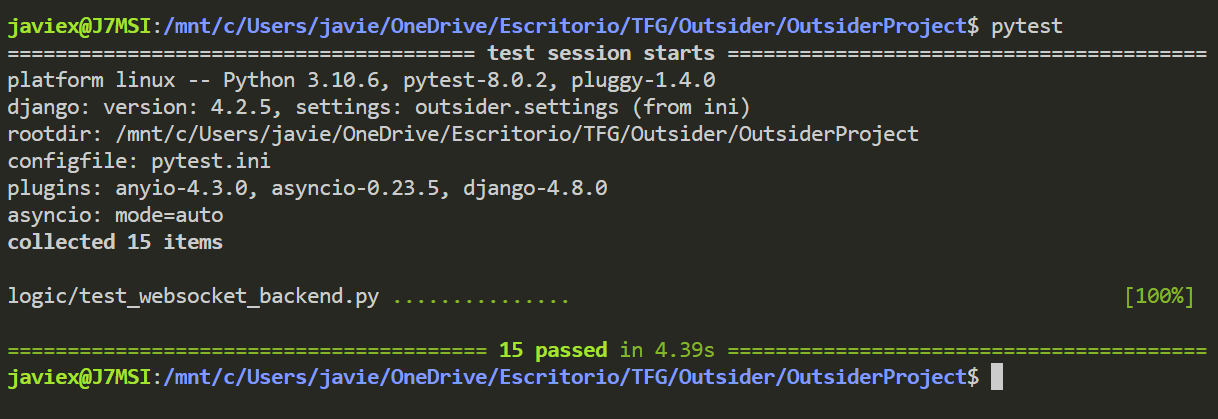
\includegraphics[width=\textwidth,clip=true]{res_testing.png}
	\caption{Ejecución de tests}
	\label{fig:res_testing}
\end{figure}
